Experimental results go here.

3. Present the results of your energy calibration and include any relevant discussion.

%\begin{figure}[h!]
%  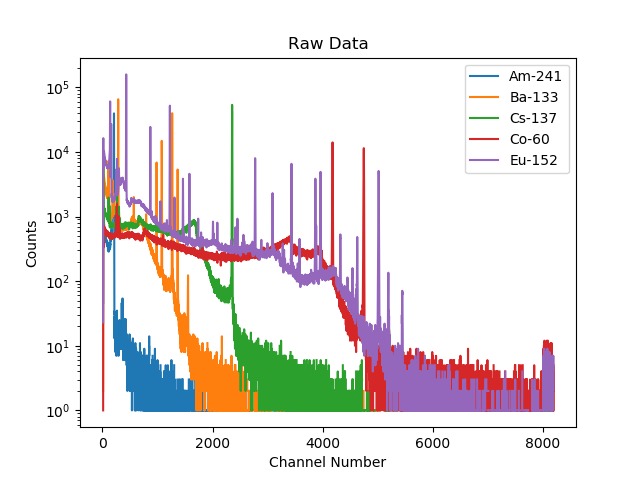
\includegraphics[width=\linewidth]{Raw_Spec.png}
%  \caption{Raw Spectrum Data.}
%  \label{fig:Raw_Spec1}
%\end{figure}

%Figure \ref{fig:Raw_Spec1} shows the uncalibrated raw spectrum data.


%\begin{figure}[h!]
%  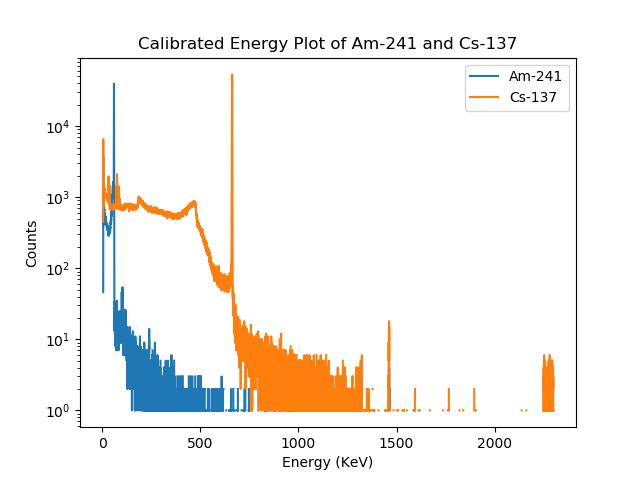
\includegraphics[width=\linewidth]{Cal_AmCs_Spec.png}
%  \caption{Calibrated Americium and Cesium Spectrum.}
%  \label{fig:Cal_AmCs_Spec1}
%\end{figure}

%Figure \ref{fig:Cal_AmCs_Spec1} shows the calibrated spectrum data for Am-241 and Cs-137.

\begin{figure}[h!]
%  \centering
  \begin{subfigure}[b]{0.6\linewidth}
    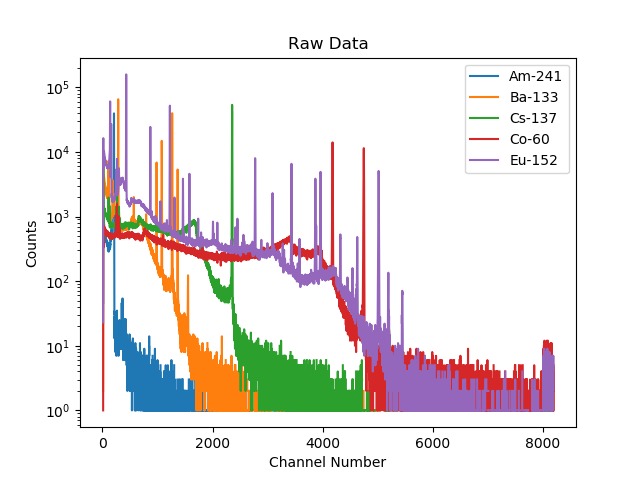
\includegraphics[width=\linewidth]{Raw_Spec.png}
    \caption{Raw Spectrum Data.}
  \end{subfigure}
  \begin{subfigure}[b]{0.6\linewidth}
    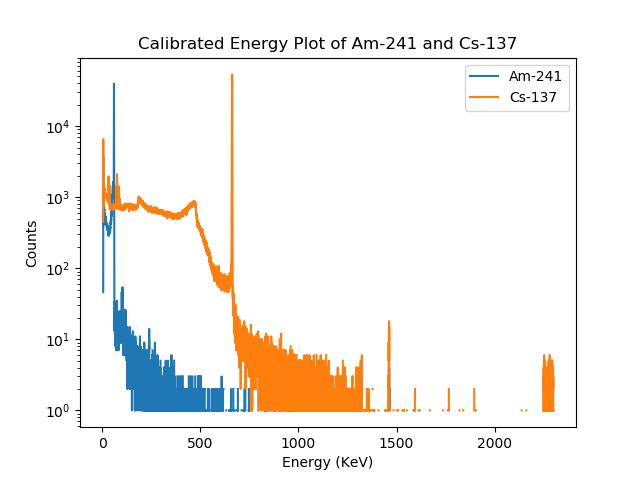
\includegraphics[width=\linewidth]{Cal_AmCs_Spec.png}
    \caption{Calibrated Am-241 and Cs-137 Spectra.}
  \end{subfigure}
  \caption{Raw data and Calibrated Spectra.}

\end{figure}

\csvautotabular{/Users/darrellstepter/repos/school/NE204/Lab0/dvstepter-lab0/images/peakdiffquant.csv}
